\documentclass{beamer}
\usetheme{Warsaw}
\usepackage{subfig}

\author{Cameron Gray}
\title{UG4 Project - IT Infrastructure Monitoring System}

\begin{document}
	\frame{\titlepage}
	\begin{frame}
		\frametitle{What is the project?}
		To build a complete, self contained system to monitor the servers and other IT infrastructure in
		small to medium organisations which may not have a dedicated IT department.
		\pause
		\begin{itemize}
			\item Provide both time series monitoring and real time alerting
			\pause
			\item Can be managed entirely from a central interface
			\pause
			\item Support for plugins to monitor specialised hardware
		\end{itemize}
	\end{frame}
		
	\begin{frame}
		\frametitle{Components}
		System is split up into 4 main components
		\begin{itemize}
			\item Agent
			\item Core
			\item Web
			\item Alerting
		\end{itemize}
	\end{frame}
	
	\begin{frame}
		\frametitle{Progress - Evaluation of Current Tools}
		Investigated current tools including Nagios, Icinga 2 and Munin and evaluated them against
		several points.
		\begin{itemize}
			\item Support for timeseries monitoring and real time alerting
			\item How they can be configured to monitor custom metrics
			\item How are alert thresholds defined
			\item How the user configures the system
			\item How dependencies are handled
		\end{itemize}
	\end{frame}
	
	\begin{frame}[t]
		\frametitle{Progress - Agent}
		Completed - Sits on machine being monitored and provides network interface to fetch data from
		plugins which are executed by the agent.
		\begin{figure}
			\includegraphics<1>[scale=0.7]{assets/agent1.png}
			\includegraphics<2>[scale=0.5]{assets/agent2.png}
			\includegraphics<3>[scale=0.5]{assets/plugin1.png}
		\end{figure}
	\end{frame}
	
	\begin{frame}
		\frametitle{Progress - Core}
		Substantial Progress - Lives on machine doing the monitoring, handles scheduling of checks and
		sends requests for data to the agents.  Multithreaded so can run checks on multiple hosts in
		parallel.
		\begin{figure}
			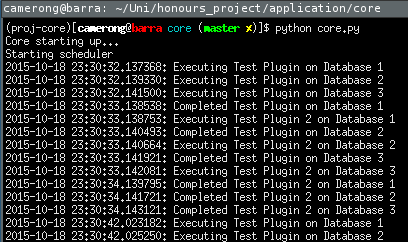
\includegraphics[scale=0.75]{assets/core1.png}
		\end{figure}
	\end{frame}
	
	\begin{frame}
		\frametitle{Progress - Web}
		\only<1>{
		Partial Implementation - Allows management of plugins, hosts, checks and schedules within the
		system.  In future will also provide management for alerting and displaying
		of collected data/graphs.
		}
		\begin{figure}
			\includegraphics<2>[scale=0.4]{assets/web_checks.png}
			\includegraphics<3>[scale=0.4]{assets/web_groups.png}
			\only<4>{
				\captionsetup[subfigure]{labelformat=empty}
				\subfloat[]{{ 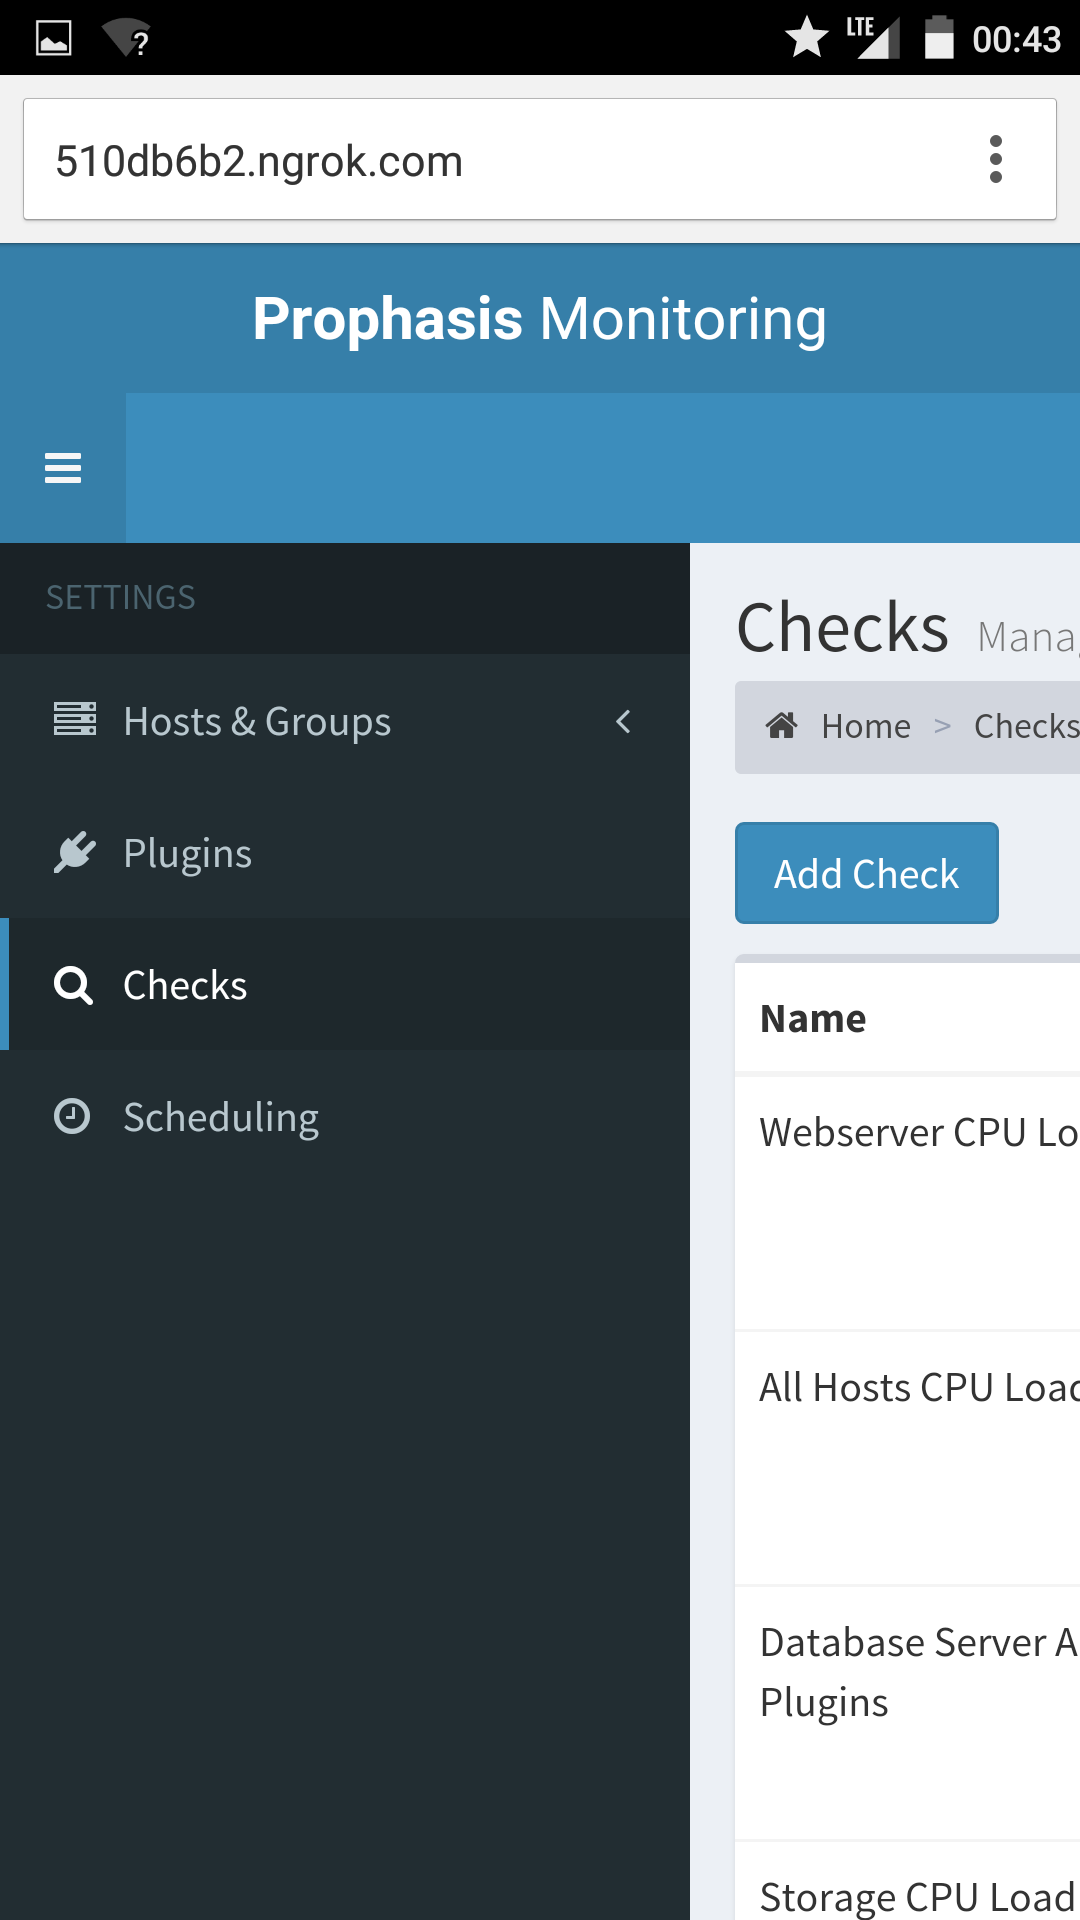
\includegraphics[scale=0.1]{assets/web_responsive_menu.png} }}
				\hfill
				\subfloat[]{{ 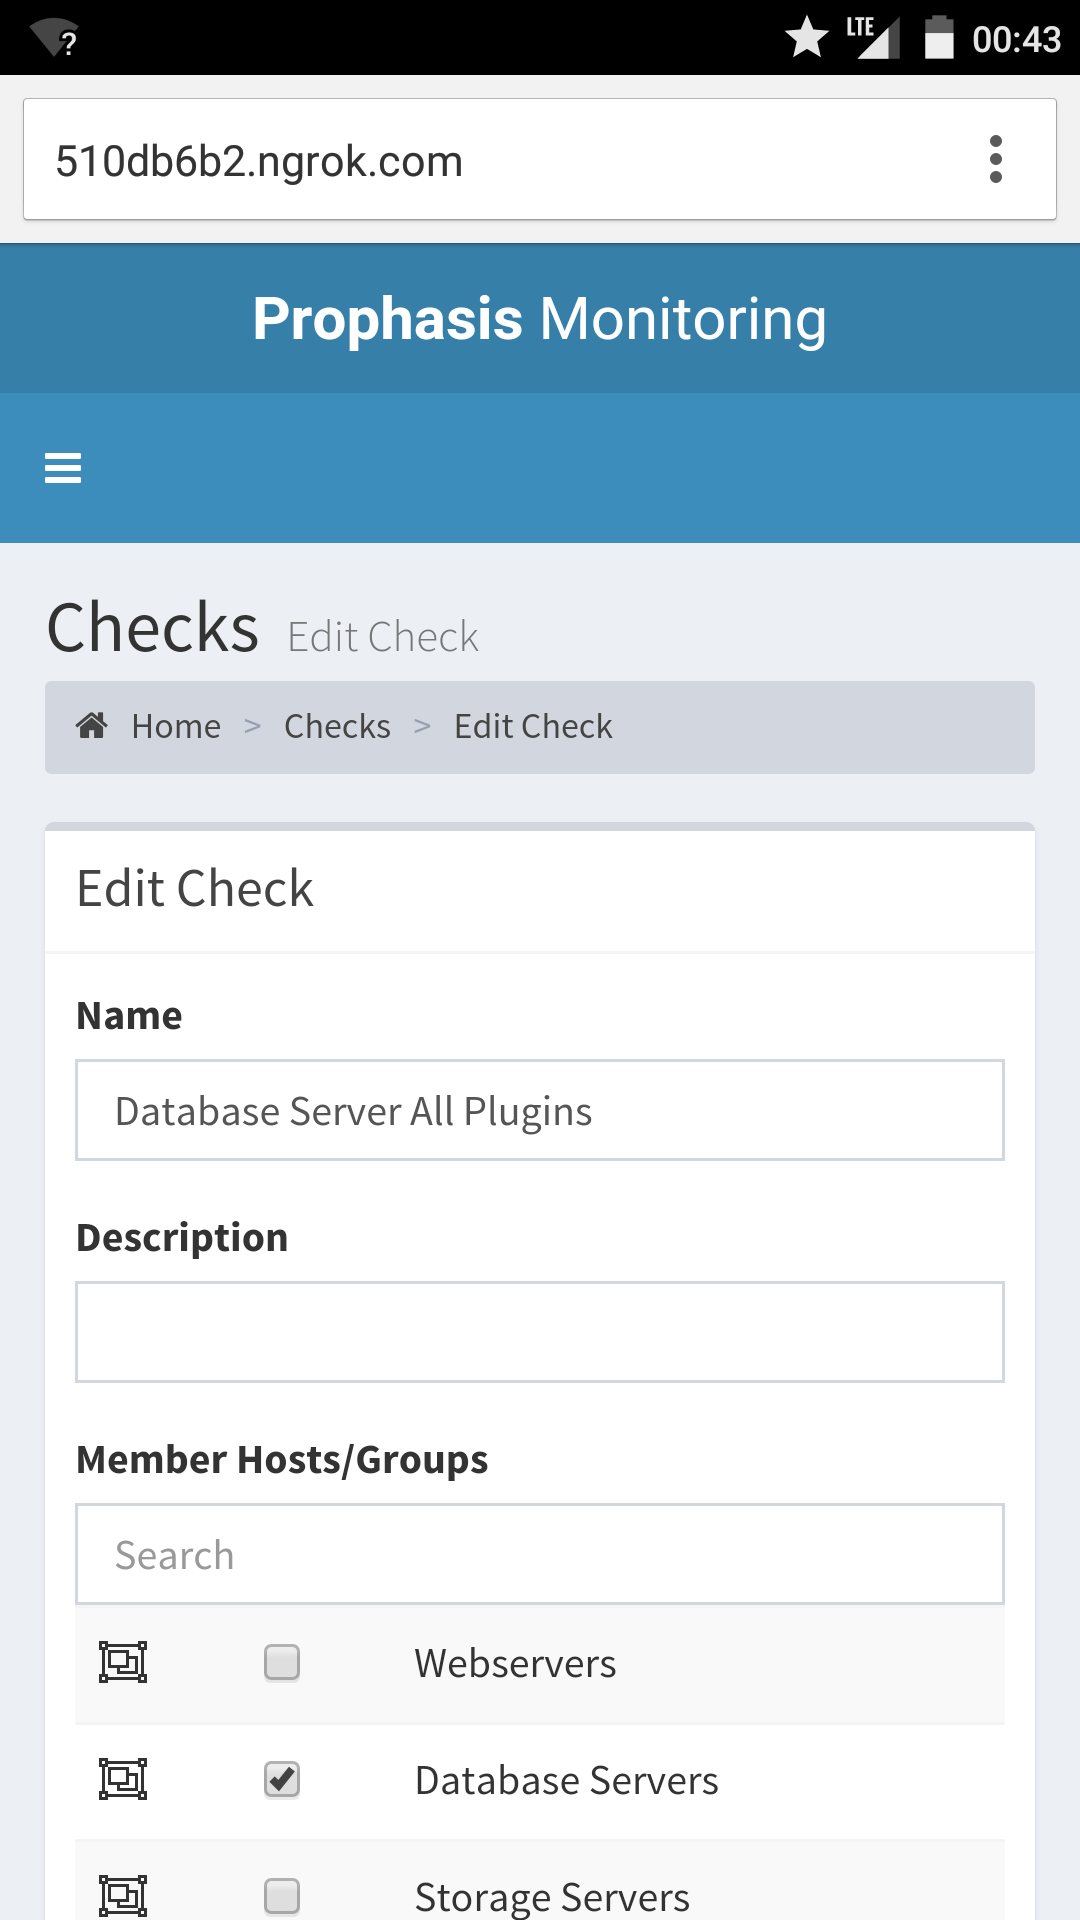
\includegraphics[scale=0.1]{assets/web_responsive_checks.png} }}
			}
		\end{figure}
	\end{frame}
	
	\begin{frame}
		\frametitle{Timeline}
		\begin{itemize}
			\item End of Week 6 (Next week)
			\begin{itemize}
				\item Initial integration - Core and agent communicating
				\item Initial test deployment on Tardis\footnotemark to collect some real data
			\end{itemize}
			\pause
			\item End of Semester 1
			\begin{itemize}
				\item Alerting complete
				\item Functional interface for visualising collected data
				\item Deploy on Tardis and gain feedback from users
			\end{itemize}
			\pause
			\item By start of Semester 2
			\begin{itemize}
				\item Work on additional features e.g. dependency support and distributed monitoring
				nodes
			\end{itemize}
			\pause 
			\item Semester 2
			\begin{itemize}
				\item Finish implementation
				\item Documentation
				\item Report
			\end{itemize}
		\end{itemize}
		
		\footnotetext[1]{http://www.tardis.ed.ac.uk/}
	\end{frame}
	
	\begin{frame}
		Questions?
	\end{frame}
\end{document}